\section{Experiments}\label{zero-shot-exp}

\subsection{Fine-tuning}
During fine-tuning, ControlNet learns a highly accurate mapping between the input and target images according to text guidance. Figure  \ref{fig:controlnet-train} shows that even the details, such as tree branches, small buildings, or windows, remain as they should. The effect of text guidance is also clearly visible in the model outputs, such as "daylight" enlightening the scene (first two columns) or "night" darkening the street (right-most column).
 
\begin{figure}[ht]
  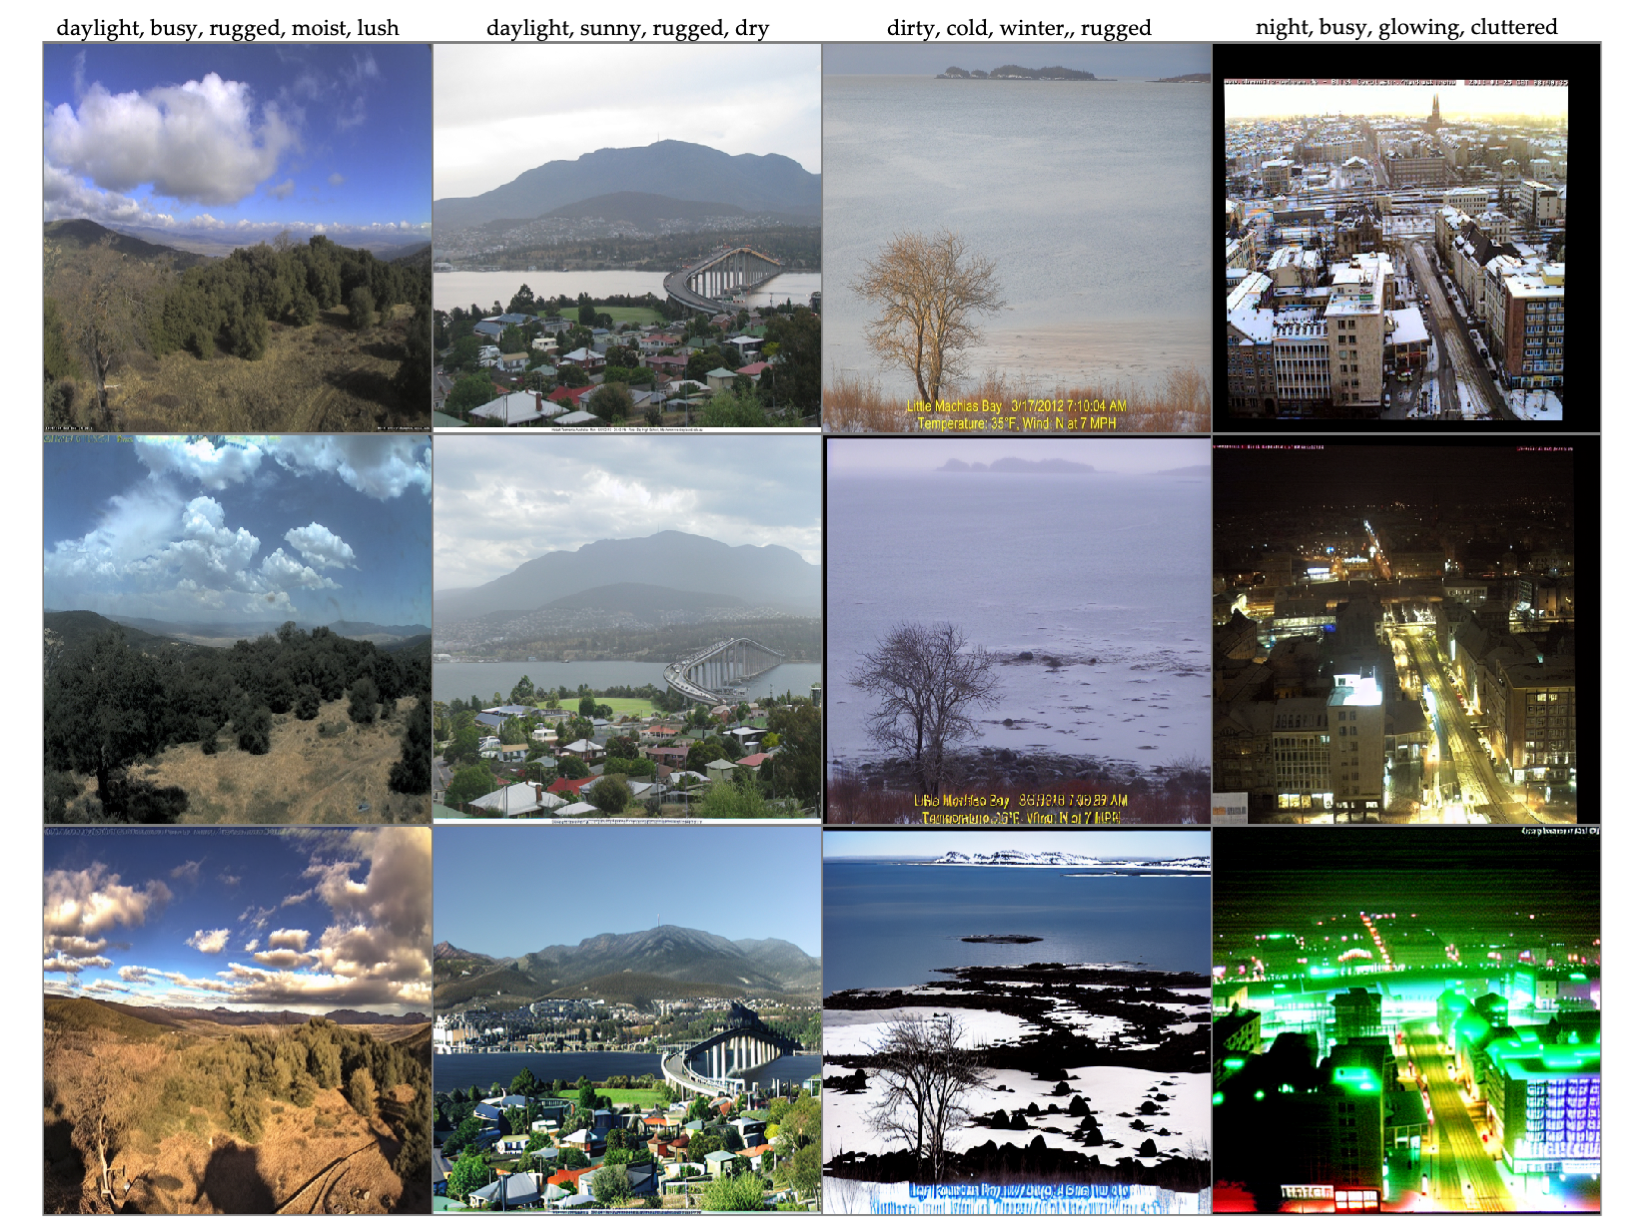
\includegraphics[width=\textwidth]{Chapters/zero-shot-tat-figs/Controlnet2.png}
  \caption{ControlNet samples from the training examples guided with the associated text prompts. Rows demonstrate input images, target images and the model outputs, in order. The subtitles indicate the attributes guiding the model.}
  \label{fig:controlnet-train}
\end{figure}

Although ControlNet performs extremely well on the training examples, its complex architecture, with a significantly high number of parameters, causes overfitting to the dataset of approximately 8000 images, leading to a performance decrease on the test dataset with losses in details and structures (Figure \ref{fig:zero-shot-comparison} - third right-most column). For instance, the car and the hut in the second row from the bottom appear to have been replaced with an unfinished construction. Another example would be the "night" prompt, where additional buildings are placed in what was supposed to be the parking area.

In terms of overfitting, the fine-tuned Stable Diffusion (second right-most column in Figure \ref{fig:zero-shot-comparison}) can preserve the wooden house in the "winter" prompt and maintain the car structure in "daylight." It can also perform content creation with respect to text guidance, comparable to ControlNet. However, both models can overdo the content creation with some newly added structures, such as clouds, covering large areas in the input image.

\subsection{Zero-shot latent diffusion}
In the zero-shot case, the similarity of the model output to the input image is controlled by the start step  $t_s$, which counts from the end step  $T$. That is, the input of the sampling process is the intermediate latent that was denoised for $t_s$ steps, starting with pure noise. I keep the total number of steps as 150 in all experiments. I also experimented with larger and smaller time steps; however, I observed that as long as the ratio of the start step to the total number of steps is the same, the results remain similar. Therefore, I only experimented with the start step to maintain the core features.


The guidance scale is another crucial parameter for the success of the zero-shot setting, as it transforms the input image according to the desired attribute. I tried four different values (10, 20, 30, 40) and observed that there is no one-size-fits-all value for all images. This also applies to the start step and poses a trade-off between the preservation of the essential content and the strength of the desired transfers. I chose the zero-shot results in Figure \ref{fig:zero-shot-comparison}  (right-most column) based on the subjective judgement of this trade-off.

\subsection{Grid search}

\begin{figure}[ht]
  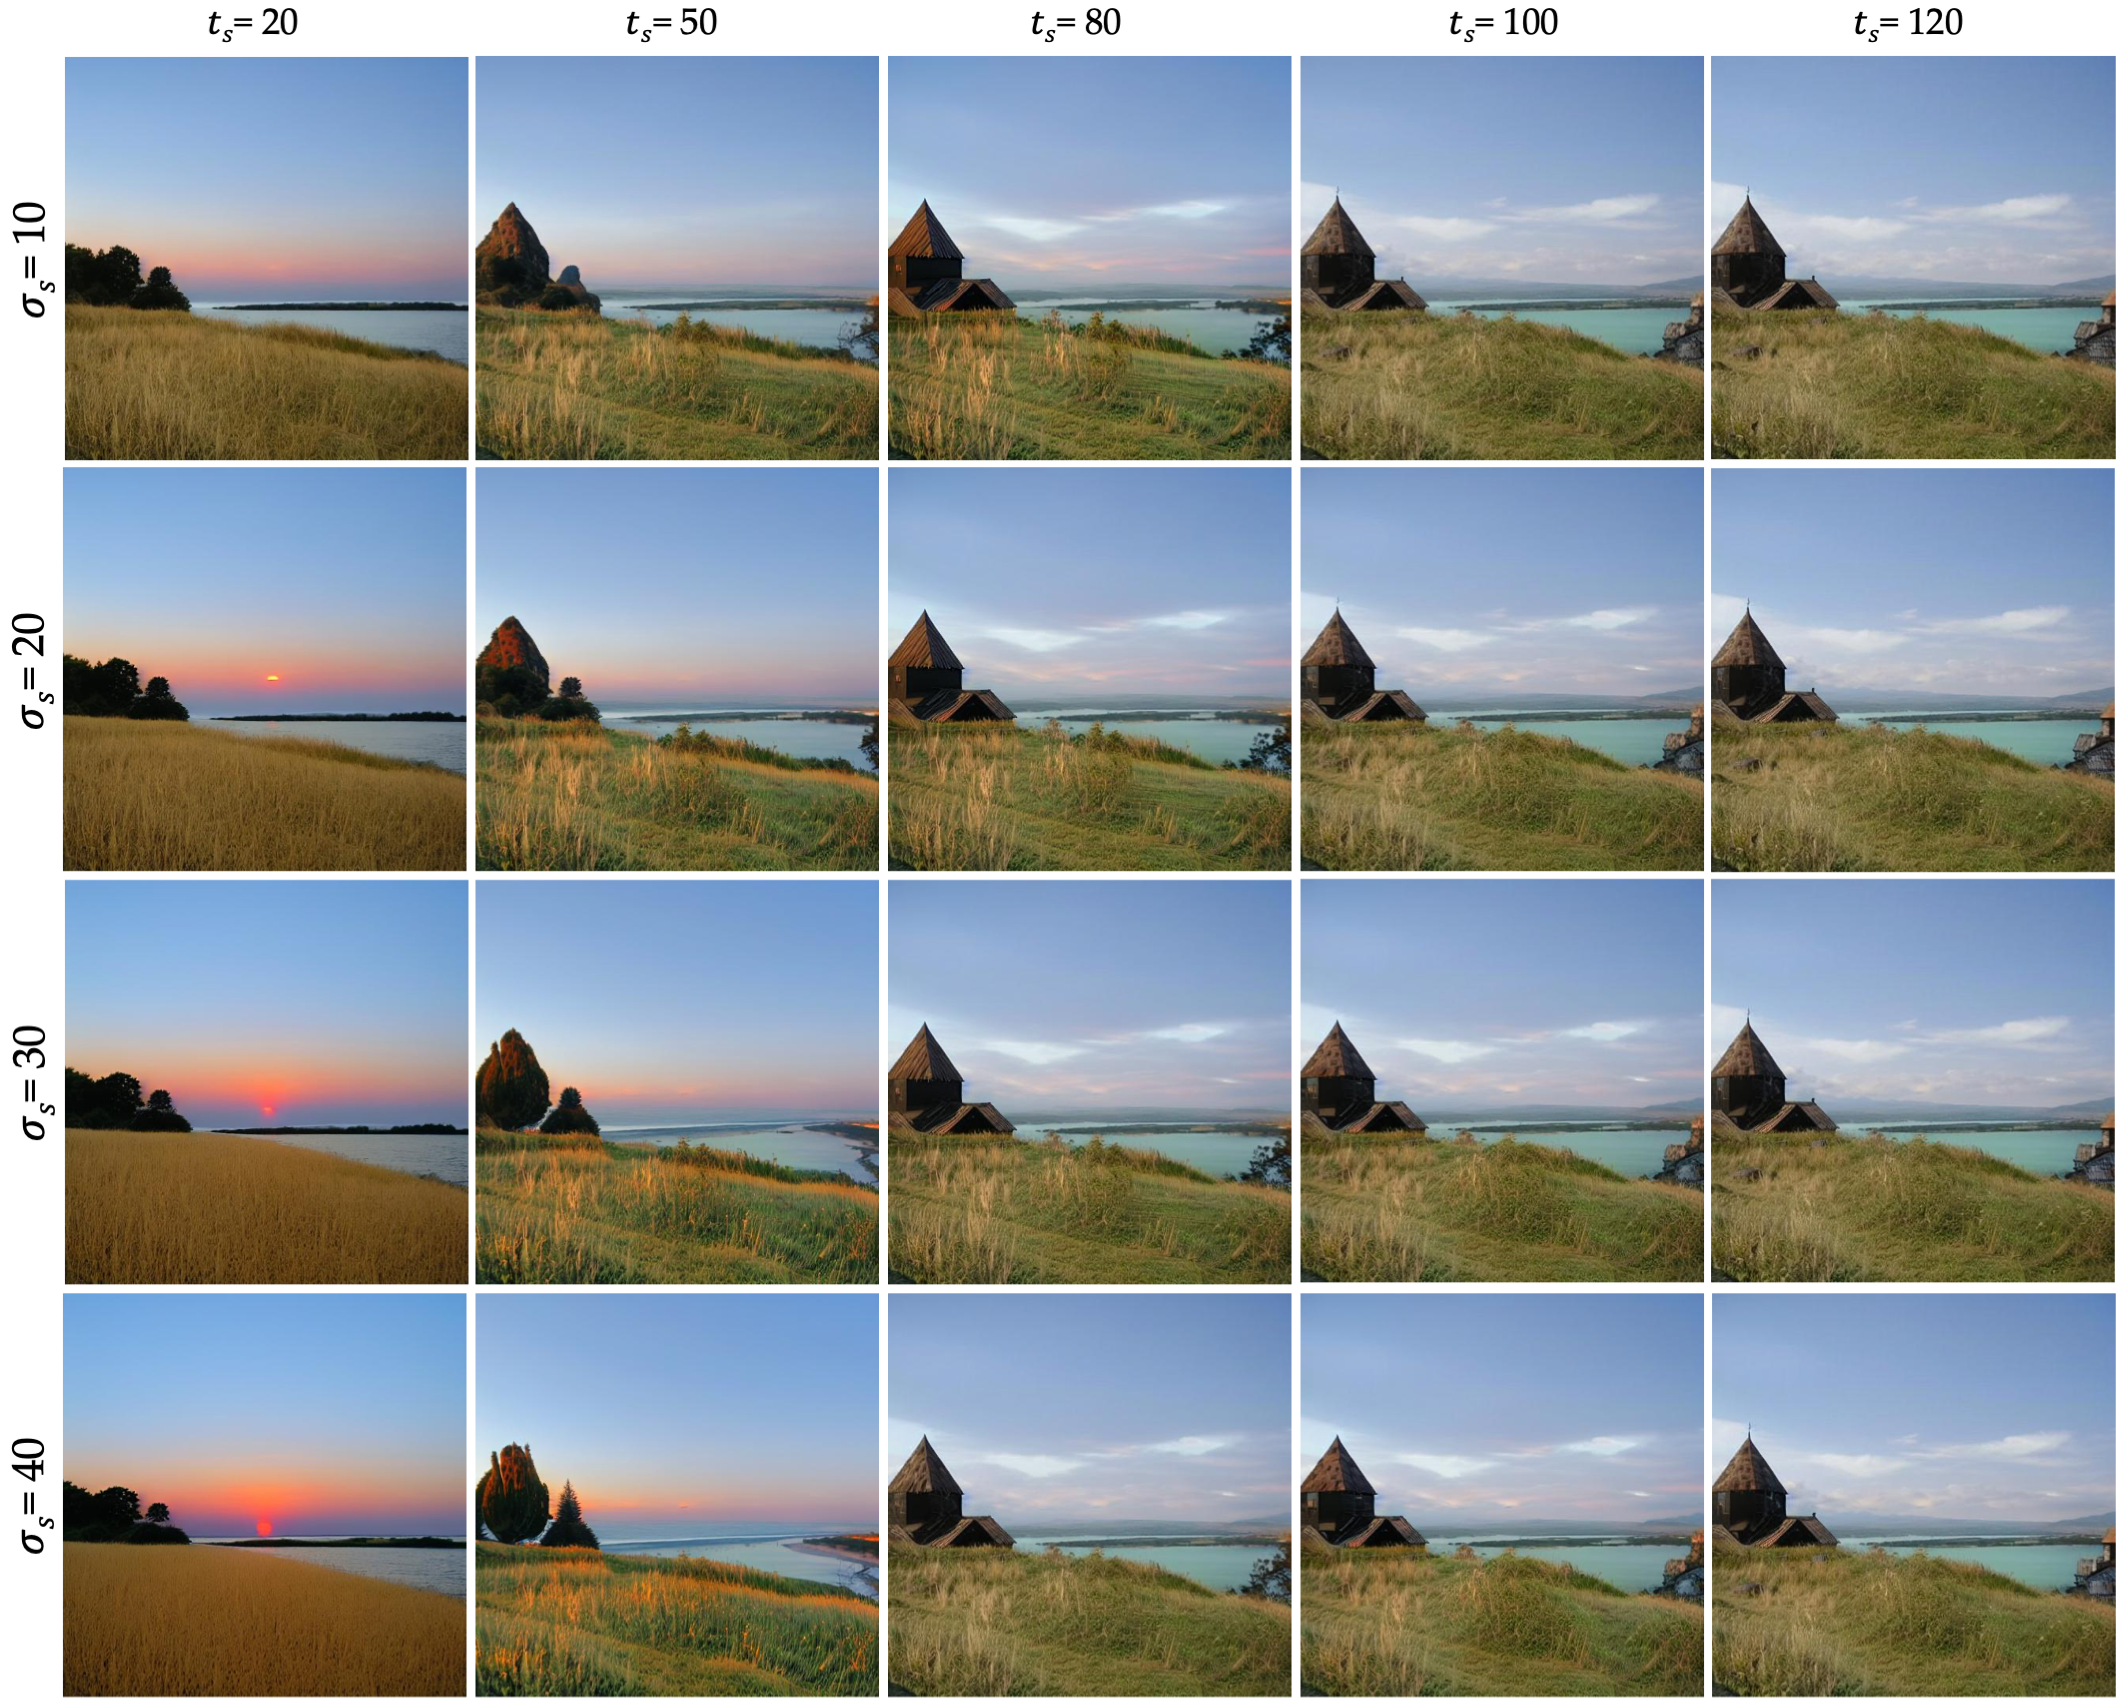
\includegraphics[width=\textwidth]{Chapters/zero-shot-tat-figs/grid-search.png}
  \caption{Grid search on DDIM inversion for the start step and the guidance scale. Here, the text prompt is "sunrise sunset".}
  \label{fig:zero-shot-grid-search}
\end{figure}

I ran an additional grid search on both parameters to find a balance between the text guidance and similarity to the input image. I experimented with $20, 50, 80, 100, 120$ for the start step out of the total number of 150 steps, and $10, 20, 30, 40$ for the guidance scale. Figure \ref{fig:zero-shot-grid-search} shows the grid search results for a test image, where we observe that increasing the guidance scale changes the appearance more strongly, whereas increasing the start step reduces the generation ability of the model.



\subsection{Qualitative comparison}
\paragraph{Baselines.} I also compare the fine-tuning and the zero-shot results with \citeauthor{laffont2014transient} \cite{laffont2014transient} and InstructPix2Pix \cite{brooks2023instructpix2pix} qualitatively. \citeauthor{laffont2014transient} \cite{laffont2014transient} learns the transforms from a pair of \textit{ Match - Target} images, as shown in the second and third columns. It has the disadvantage of requiring two additional images. On the other hand, InstructPix2Pix \cite{brooks2023instructpix2pix} is a diffusion-based model designed to edit images according to instructions. It is fine-tuned with a large dataset of image-target pairs along with their associated instructions. To adapt their model to our task, I convert the attributes to instructions by adding "make it" to the front of the adjective version of the attribute. For instance, if the prompt is initially "summer," then the InstructPix2Pix input becomes "make it sunny." Without this adjustment, I observed little to no changes in the input images.


 
 \begin{figure}[ht]
  \includegraphics[width=\textwidth]{Chapters/zero-shot-tat-figs/zeros-shot-qual-comp-updated.pdf}
  \caption{Qualitative comparison with the baseline methods on the test images of the Transient Attribute Dataset \cite{laffont2014transient}. Additional results can be found in Appendix \ref{TAT:add_res}.}
  \label{fig:zero-shot-comparison}
\end{figure}

Figure \ref{fig:zero-shot-comparison} shows that Zero-shot (right-most column) overall attains compelling results, comparable with InstructPix2Pix (fifth column). It maintains the core structures while transferring the target attributes to the input image. \citeauthor{laffont2014transient} \cite{laffont2014transient} can also accurately capture the transfer, but their edits remain limited to the \textit{Match - Target} pair, being unable to add some additional content, such as snow or raindrops. Both ControlNet (third column from the right) and Stable Diffusion (second from the right) are better capable of generating new content (clouds, snow, daylight, etc.). However, these models are less reliable in terms of content preservation. 

